\documentclass{beamer}
\mode<presentation>
{
\usetheme{Rochester}
\setbeamercovered{transparent}
\useoutertheme{smoothbars}
}
\addtobeamertemplate{footline}{\insertframenumber/\inserttotalframenumber}

\usepackage[utf8]{inputenc} \usepackage[english]{babel}
\usepackage{graphicx} \usepackage{geometry}
\usepackage{pifont}
\usepackage{hyperref}
\usepackage{tikz}
\usepackage{fancyvrb}
\DefineVerbatimEnvironment{verbatim}{Verbatim}{formatcom=\color{blue}}
%\usepackage{minted}

%\newminted{python}{fontsize=\scriptsize,linenos}
%\newminted{python3}{fontsize=\tiny,linenos}


\newcommand{\E}[1]{{\textbf{#1}}}
\newcommand{\C}[1]{{\color{red}\texttt{#1}}}
\definecolor{mygreen}{cmyk}{0.888,0,0.888,0.298}
\newcommand{\G}[1]{{\color{mygreen}{#1}}}
\newcommand{\B}[1]{{\color{blue}{#1}}}
\newcommand{\ar}{\ding{220} }
\newcommand{\todo}[1]{{\colorbox{yellow}{\color{fg}#1}}}


\title{VM5k and DVMS on Grid'5000}
\subtitle{Deploying and Managing Thousands of Virtual Machines on Hundreds of Nodes Distributed Geographically}

% - Use the \inst{?} command only if the authors have different
%   affiliation.
%\author{F.~Author\inst{1} \and S.~Another\inst{2}}
\author{Javier Pastor\inst{1} \and Laurent Pouilloux\inst{2}}

% - Use the \inst command only if there are several affiliations.
% - Keep it simple, no one is interested in your street address.
\institute[Hemera]
{
\inst{1}%
Héméra Phd\\
ASCOLA - Mines Nantes / Inria
\and
\inst{2}%
Hemera Engineer\\
Inria / ENS Lyon}

\date[G5K School 2014]{18-06-2014 / Grid'5000 School}


% This is only inserted into the PDF information catalog. Can be left
% out.
\subject{VM5K_DVMS}



% If you have a file called "university-logo-filename.xxx", where xxx
% is a graphic format that can be processed by latex or pdflatex,
% resp., then you can add a logo as follows:

%\pgfdeclareimage[height=0.5cm]{university-logo}{logo_inria.jpg}
%\logo{\pgfuseimage{university-logo}}


\begin{document}

\begin{frame}
\titlepage
\end{frame}


\begin{frame}{Context}
Cloud computing has become very popular.
\begin{itemize}
\item Ever-increasing demand $\Rightarrow$ ever-increasing
infrastructure size.
\item PB: scalability, reliability, energy but also security,
juridiction and network overhead.
\item Decentralise the production of computing ressources
(Discovery project, http://beyondtheclouds.github.io/)
\end{itemize}
\end{frame}


\begin{frame}{Scientific question}
Discovery: leverage the concept of micro/nano
datacenters [Greenberg2009] geographically spread.
$\Rightarrow$ nodes can be far from each other.
\begin{itemize}
\item And we want to maximise cooperation between close
nodes/micro DCs.
\item Example: The DVMS case.
\end{itemize}
\end{frame}


{
\usebackgroundtemplate{%
\tikz[overlay,remember picture] \node[opacity=1, at=(current page.center)] {
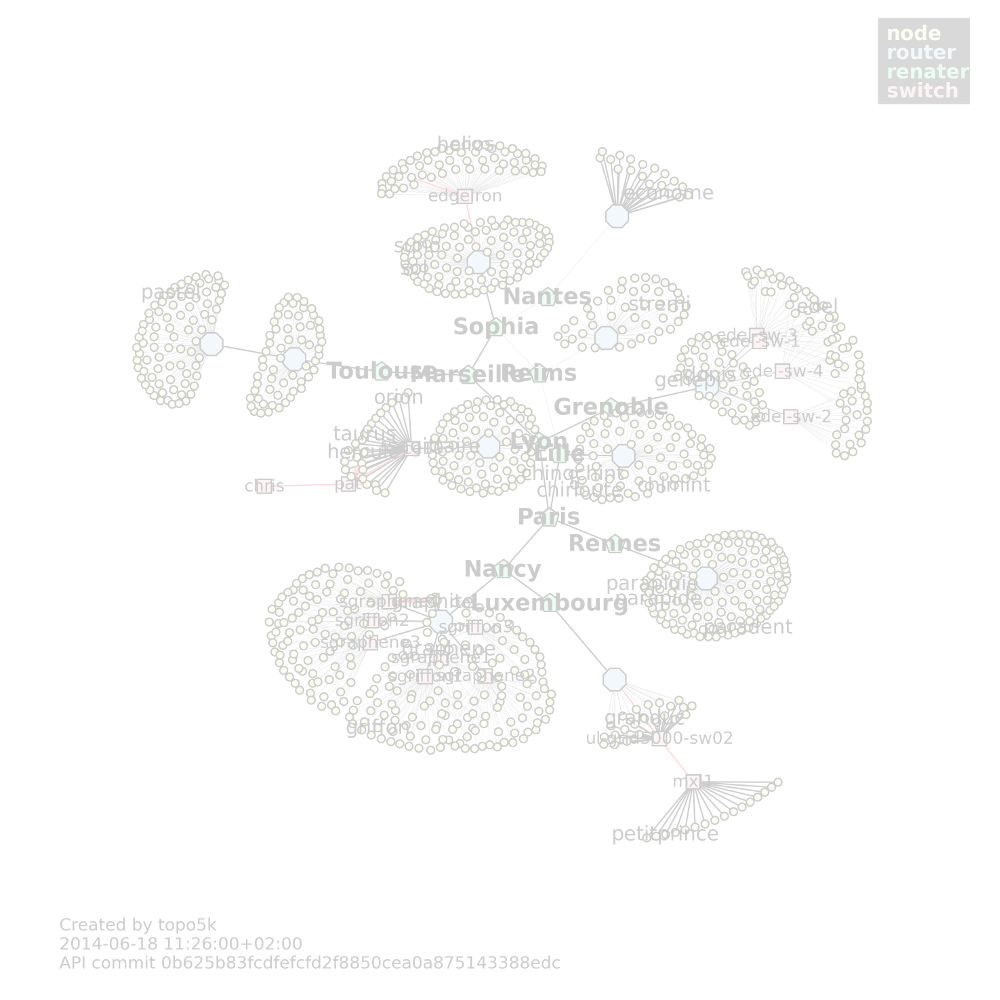
\includegraphics[height=0.9\paperheight,width=0.9\paperwidth,keepaspectratio]{topo5k.png}};
}
\begin{frame}{Grid'5000 as a testbed}
\begin{itemize}
\item renater interconnected network
\item various hardware
\item KaVLAN
\item experimentfull stack control 
\end{itemize}
\end{frame}
}




\begin{frame}{Experimental Workflow}
\begin{enumerate}
\item reserve many nodes on different sites, with a global-KaVLAN
\item deploy thousants of Virtual Machines
\item initiate stress process on them
\item install DVMS
\item use vivaldi to compute hosts distances
\item generate random stress on the virtual machiens
\item collect results
\end{enumerate}
\end{frame}

\begin{frame}{Automatic time slot selection}
\end{frame}

\begin{frame}{Virtual Machines deployment}
\end{frame}

\begin{frame}{Stress initialization}
\end{frame}

\begin{frame}{Vivaldi}
\end{frame}

\begin{frame}{DVMS}
\end{frame}

\begin{frame}{Live visualization}
\end{frame}

\begin{frame}{Results Analysis}
\end{frame}

\begin{frame}{Conclusion}
* publi Europar
* github repository
\end{frame}


\end{document}
